\appendix
\section{Errorbars for Gini index}\label{Appendix A}
\textit{Bootstrap} method\cite{bootstrap} is used to compute
\textit{Gini index}' mean and error: while for the former the process
is pretty straigthforward, this is not the case for the latter.
The average fraction of users reached distribution is asymmetrical and, in general,
non-normal. We consider two different types of error:
given N samples ${x_1,...,x_N}$ whose mean is $\mu$,
\textit{correct standard deviation} is:
$\sigma=\sqrt{\frac{\sum_{i=1}^{i=N}(x_i - \mu)^2}{N-1}}$.\\
\textit{Quantile Standard Error}\cite{quantile} (QSE), instead,
estimates the error by considering the fraction of samples
falling within a certain interval: the whole distribution is
divided in equal parts by a certain amount of ``quantiles''.\\
For example, in a Normal distribution, the interval
$[\mu -\sigma, \mu +\sigma]$ ``covers'' approximately $68\%$
of the samples.
In ``quantiles'' terms (percentiles in this case), our errorbar
starts from the $16^{th}$ percentile and ends in the $84^{th}$
percentile.\\
standard deviation, computed for non-normal distributions does
not follow this property in general: to preserve it, we can compute QSE with
the previous choice of quantiles, just by looking at the cumulative
distribution, when values 0.16 and 0.84 are reached.
\begin{table}[htpb]
  \centering
  \begin{tabular}{rc|cc}
    \toprule
    \multicolumn{2}{c}{\textit{quantile}} & $16\%$ & $84\%$ \\
    \midrule
    Number & \SI{10}{} & \SI{1.3e-2}{}  & \SI{8.57e-3}{} \\
    of & \SI{e3}{} & \SI{2.39e-2}{} & \SI{5.64e-3}{} \\
    boot & \SI{e5}{} & \SI{2.36e-2}{} & \SI{5.22e-3}{} \\
    samples & \SI{e7}{} & \SI{2.36e-2}{} & \SI{5.34e-3}{} \\
    \bottomrule
  \end{tabular}
  \caption{Quantile errors.}
  \label{tab:quantile}
\end{table}
\begin{figure}[h!]
  \centering
  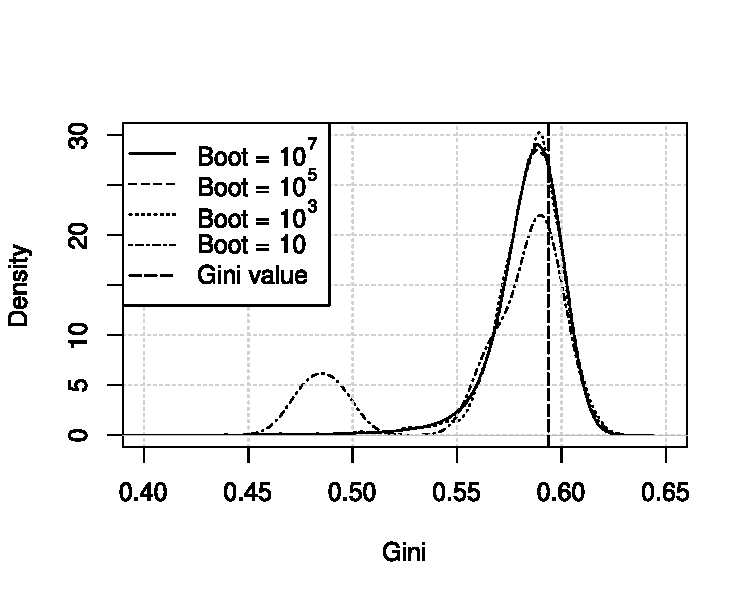
\includegraphics[width=.8\columnwidth]{img/bootstrap.pdf}
  \caption[Average Gini index bootstrap plot.]{Several bootstraps with different sampling size.
    After $10^5$ samplings the distribution is pretty much the same:
    hence we chose a size of $10^5$ to compute average Gini Index.}
  \label{fig:bootstrap}
\end{figure}
\\
The overall error is divided twofold: ``rightmost'' and ``leftmost''
the mean. For every part of the interval, we pick the ``largest''
between standard deviation and QSE, see figure
(\ref{fig:gausssigma}): this conservative approach avoids
underestimations in both directions.
%
\section{Asymmetric errorbars fitting}\label{Appendix B}
The aim of a standard fitting problem is to find a function which
reproduces experimental observations.
Let $f_{\theta}$ be the candidate function:
$\theta=(\theta_1,...,\theta_m)$ is a vector of $m$ parameters which
completely determine function's values.
The optimization is performed with respect to $\theta$.\\
Given N datapoints with coordinates ${(x_i,y_i)}$ and y-errorbars
$\sigma_i$ for $i$=1,...,N, the usual optimization function for
\textit{weighted interpolation}\cite{interpolation} is:
$$
E(\theta)= \sum_{i=1}^{N} \frac{(f_{\theta}(x_i)-y_i)^2}{\sigma_{i}^2}
$$
However, this formula is only applicable to gaussian errors,
expressed by the standard deviation: in the problem we are facing,
errorbars are not even symmetric.
We have developed an approximate optimization function which counts
in this asymmetry.
In a weighted interpolation, the weight is the square inverse of the
standard deviation: the ``shortest'' the errorbar, the closest will
be $f(x_i)$ to $y_i$.
It might be an idea to split the error in two contributions,
to be ``activated'' if the function value is greater or lower
than the experimental value.
Let $a$ and $b$ be, respectively, the upper and lower portion of errorbars
compared to the mean point $p$ (as shown in figure~\ref{fig:errors});
the optimization function for \textit{asymmetric
  errobars interpolation} is:
$$ E= \sum_{i=1}^{N} \frac{(f(x_i)-y_i)^2}{a^{2}\mathcal{H}(f(x_i)-y_i)+b^{2}\mathcal{H}(y_i-f(x_i))} $$
$\mathcal{H}(x)$ is the \textit{Heaviside function},
$$\mathcal{H}(x):=\frac{\mathrm{d}}{\mathrm{d}x}\mathrm{max}
\{x,0\}:=\int_{-\infty}^x \delta (s) \mathrm{d}s$$ whose value
is zero for negative argument and one for positive argument.\\
The optimization is performed by an R implementation\cite{Roptim}
of \textit{Nelder-Mead algorithm},\cite{neldermeadoriginal}
also known as \textit{downhill simplex method} or
\textit{amoeba}.\cite{neldermeadnumrec}\\
This algorithm is particularly appropriate for non-linear
optimization with many local minima.
\begin{figure}[h!]
  \centering
  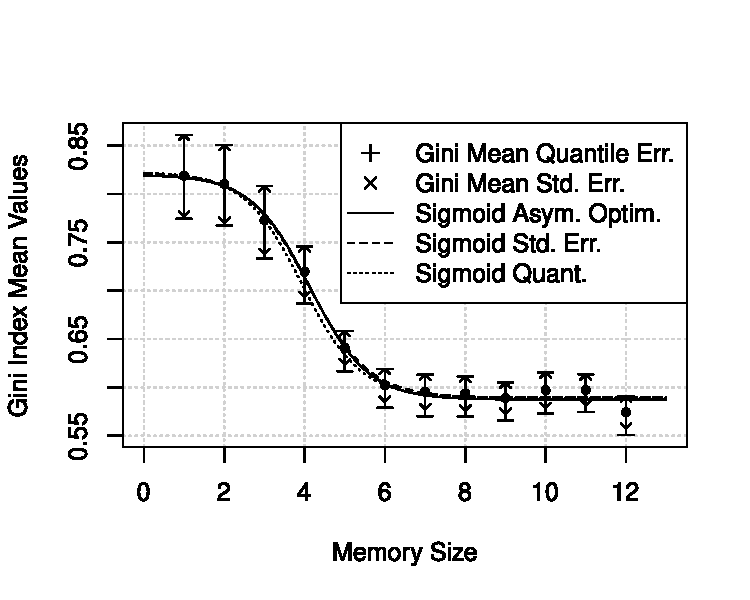
\includegraphics[width=.8\columnwidth]{img/appendix.pdf}
  \caption[Three different regressions for Gini index.]{Three different regressions are shown for gini index over
    memory length plot: optimizations are performed using standard
    deviation, quantiles and asymmetric errorbars.}
  \label{fig:gausssigma}
\end{figure}
\begin{figure}[h!]
  \centering
  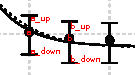
\includegraphics[width=.5\columnwidth]{img/err.pdf}
  \caption{Asymmetric errorbars.}
  \label{fig:errors}
\end{figure}
\\
